\section{光谱表示}\label{sec:光谱表示}

真实世界物体的SPD可能极其复杂;
\reffig{5.1}展示了荧光灯发光的频谱分布和柠檬皮反射率的频谱分布图。
用SPD做计算的渲染器需要紧实、高效且准确的方式表示像这样的函数。
实践中,可能需要在这些特性间作取舍。
\begin{figure}[htbp]
    \centering
    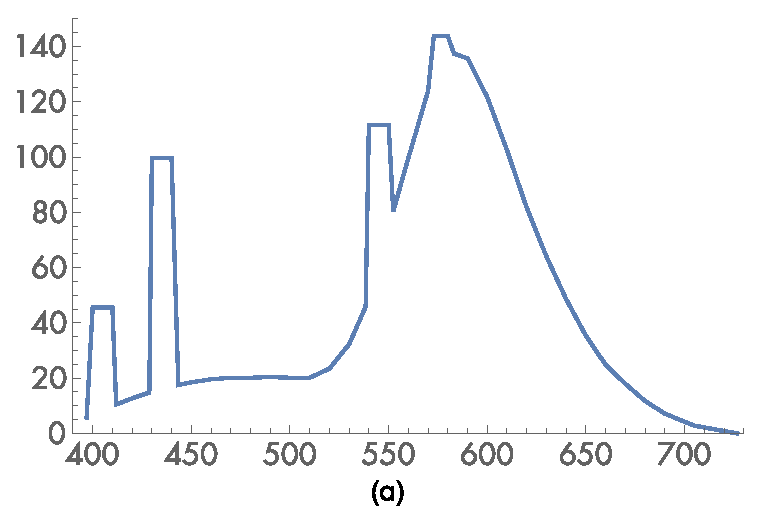
\includegraphics[width=0.45\linewidth]{chap05/fluorescent-spd.eps}\,\nolinebreak
    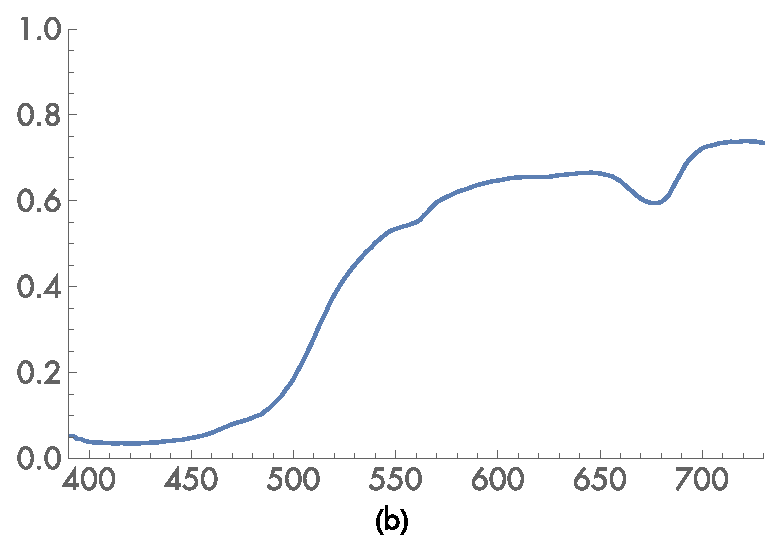
\includegraphics[width=0.45\linewidth]{chap05/lemonskin-spd.eps}
    \caption{(a)荧光灯的频谱分布和(b)柠檬皮的反射率。
    波长400nm左右是偏蓝光,而波长中段是绿色和黄色,波长700nm左右是红光。
    荧光灯的SPD甚至比这里展示的更加尖锐,SPD可归入到10nm范围内;
    它实际上是在单个离散频率上发出大量光。}
    \label{fig:5.1}
\end{figure}

研究这些问题的一般框架可以基于寻找
优良\keyindex{基函数}{basis function}{}以表示SPD的问题来开发。
基函数背后的思想是将可能的SPD函数的无限维空间映射到系数$c_i\in\mathbb{R}$的低维空间。
例如,一个平凡的基函数是常函数$B(\lambda)=1$。
任意SPD可以用等于其平均值的单个系数$c$以该基表示,
这样其近似就为$cB(\lambda)=c$。
很明显这是个很差的近似,因为大多数SPD都比这单个基函数所能准确表示的复杂得多。

在计算机图形学中已经为光谱表示研究了许多不同的基函数;
“扩展阅读”一节引用了关于该话题的许多文献和更多资源。
不同基函数集在关键运算上能提供截然不同的取舍,例如
将任意SPD转换为系数集(将其投影到基上)、
为由基表示的两个SPD之积给定的SPD计算系数等。
本章中,我们将介绍pbrt中可用于光谱的两种表示:\refvar{RGBSpectrum}{},
它遵循经典计算机图形学实践中用表示红、绿和蓝色混合的系数来表示SPD的做法,
以及\refvar{SampledSpectrum}{},它将SPD表示为在一个波长范围上采样点集。

\subsection{光谱类型}\label{sub:光谱类型}
整个pbrt中,我们都根据\refvar{Spectrum}{}类型
用一组特定内建运算符(加法、乘法等)仔细实现涉及SPD的全部计算。
\refvar{Spectrum}{}类型隐藏了所用特定光谱表示的细节,
这样改变系统的这些细节只需要改变\refvar{Spectrum}{}的实现;其他代码可保存不变。
\refvar{Spectrum}{}类型的实现在文件\href{https://github.com/mmp/pbrt-v3/blob/master/src/core/spectrum.h}{\ttfamily core/spectrum.h}和
\href{https://github.com/mmp/pbrt-v3/blob/master/src/core/spectrum.cpp}{\ttfamily core/spectrum.cpp}中。

pbrt中为\refvar{Spectrum}{}类型选择使用哪种光谱表示
在文件\href{https://github.com/mmp/pbrt-v3/blob/master/src/core/pbrt.h}{\ttfamily core/pbrt.h}中
由{\ttfamily typedef}完成。
pbrt默认使用更高效但不太精确的RGB表示。
\begin{lstlisting}
`\initcode{Global Forward Declarations}{=}\initnext{GlobalForwardDeclarations}`
typedef `\refvar{RGBSpectrum}{}` `\initvar{Spectrum}{}`;
// typedef \refvar{SampledSpectrum}{} Spectrum;
\end{lstlisting}

我们还没有把系统编写成在运行时解析选用哪个\refvar{Spectrum}{}表示;
为了切换到不同的表示,整个系统必须重新编译。
这一设计的一个优点是许多各种\refvar{Spectrum}{}方法可以实现为
能被编译器内联\sidenote{译者注:原文inlined。}的短函数,而不是弄成
需要通过相对较慢的虚拟方法调用机制唤起的独立运行函数。
内联像这样的常用短函数能给出性能上的巨大提升。
第二个优点是系统中持有\refvar{Spectrum}{}类型实例的结构可以直接保有它们
而不需要在运行时基于所选的光谱表示动态地分配它们。

\subsection{系数光谱实现}\label{sub:系数光谱实现}
本章实现的两种表示都基于排序固定数目的SPD样本。
因此,
\begin{lstlisting}
`\initcode{Spectrum Declarations}{=}\initnext{SpectrumDeclarations}`
template <int `\initvar{nSpectrumSamples}{}`> class `\initvar{CoefficientSpectrum}{}` {
public:
    `\refcode{CoefficientSpectrum Public Methods}{}`
    `\refcode{CoefficientSpectrum Public Data}{}`
protected:
    `\refcode{CoefficientSpectrum Protected Data}{}`
};
\end{lstlisting}

\begin{lstlisting}
`\initcode{CoefficientSpectrum Public Methods}{=}\initnext{CoefficientSpectrumPublicMethods}`
`\refvar{CoefficientSpectrum}{}`(`\refvar{Float}{}` v = 0.f) {
    for (int i = 0; i < `\refvar{nSpectrumSamples}{}`; ++i)
        `\refvar[CoefficientSpectrum::c]{c}{}`[i] = v;
}
\end{lstlisting}

\begin{lstlisting}
`\initcode{CoefficientSpectrum Protected Data}{=}`
`\refvar{Float}{}` `\initvar[CoefficientSpectrum::c]{c}{}`[`\refvar{nSpectrumSamples}{}`];
\end{lstlisting}

\begin{lstlisting}
`\refcode{CoefficientSpectrum Public Methods}{+=}\lastnext{CoefficientSpectrumPublicMethods}`
bool `\initvar{IsBlack}{}`() const {
    for (int i = 0; i < `\refvar{nSpectrumSamples}{}`; ++i)
        if (`\refvar[CoefficientSpectrum::c]{c}{}`[i] != 0.) return false;
    return true;
}
\end{lstlisting}